\section{Обработка результатов измерений}

\begin{enumerate}
    \item Перевести показания лабораторного барометра из миллиметров 
    ртутного столба в паскали: 
    \begin{equation}
        p_0(Па) =  p_0(мм. рт. ст.) \cdot \rho g
    \end{equation}
    Здесь $\rho = 13{\,}551 \frac{кг}{м^3}$ "--- плотность 
    ртути, $g = 9{,}819 \frac{м}{с^2}$ "--- ускорение свободного 
    падения на широте Санкт-Петербурга.
    
    \item Для каждой из таблиц 1.1--1.5 вычислить давление газа $P$ по формуле
    \begin{equation}
        P = P_0 + \frac{\Delta p_1 + \Delta p_2}2
    \end{equation}
    обратное давление $\frac1P$ и заполнить пятую и шестую колонки таблиц.
    
    \begin{center}
    Таблица 1.1. Зависимость давления от объема при температуре $t_1 = 14{,}5^{\circ}C$
    \nopagebreak
    
    \begin{tabular}{|c|c|c|c|c|c|c|c|}
\hline
phi & 1 & 3 & 5 & 7 & 9 & 11 & 13\\
\hline
1 & 159 & 156 & 160 & 156 & 161 & 159 & 159\\
\hline
2 & 139 & 136 & 137 & 138 & 136 & 138 & 139\\
\hline
4 & 98 & 100 & 98 & 96 & 99 & 100 & 98\\
\hline
6 & 62 & 63 & 65 & 61 & 61 & 59 & 59\\
\hline
8 & 27 & 30 & 24 & 27 & 26 & 27 & 25\\
\hline
9 & 10 & 11 & 10 & 12 & 12 & 9 & 9\\
\hline
\end{tabular}
\par

    \vspace{0.1cm}
\end{center}

\begin{center}
    Таблица 1.2. Зависимость давления от объема при температуре $t_2 = 24{,}4^{\circ}C$
    \nopagebreak
    
    \begin{tabular}{|c|c|c|c|c|c|}
\hline
\No & $V_ц$, мл & $\Delta P_1$, кПа & $\Delta P_2$, кПа & $P$, кПа & $\frac1P$, кПа${}^{-1}$\\
\hline
1 & 50 & 7,3 & 7 & 108,938810785 & 0,009179465\\
\hline
2 & 60 & -7,7 & -6,1 & 94,888810785 & 0,0105386504\\
\hline
3 & 70 & -17,8 & -17,9 & 83,938810785 & 0,0119134402\\
\hline
4 & 80 & -27,2 & -27,5 & 74,438810785 & 0,0134338524\\
\hline
5 & 90 & -34,7 & -35 & 66,938810785 & 0,0149390165\\
\hline
6 & 100 & -40,9 & -41 & 60,838810785 & 0,0164368762\\
\hline
7 & 110 & -46,1 & -46,2 & 55,638810785 & 0,0179730657\\
\hline
8 & 120 & -50,4 & -50,5 & 51,338810785 & 0,0194784411\\
\hline
9 & 130 & -54 & -54 & 47,788810785 & 0,0209254004\\
\hline
10 & 140 & -57,3 & -57,4 & 44,438810785 & 0,0225028524\\
\hline
\end{tabular}
\par

    \vspace{0.1cm}
\end{center}

\begin{center}
    Таблица 1.3. Зависимость давления от объема при температуре $t_3 = 33^{\circ}C$
    \nopagebreak
    
    Таблица 2.3
\begin{tabular}{|c|c|c|c|c|c|c|}
    \hline
    \multirow{2}{*}{\No} & \multicolumn{4}{|c|}{измеренные величины} & \multicolumn{2}{c|}{рассчитанные величины}\\ \cline{2-7}
    & $x_1$, м & $x_2$, м & $t_1$, с & $t_2$, с & $2(x_2-x_1)$, м & $t_2^2-t_1^2$, $c^2$\\
    \hline
    1 & 0,15 & 0,7 & 2,1 & 4,9 & 1,1 & 19,6\\
    \hline
    2 & 0,15 & 0,7 & 2,3 & 5,3 & 1,1 & 22,8\\
    \hline
    3 & 0,15 & 0,7 & 2,3 & 5,3 & 1,1 & 22,8\\
    \hline
    4 & 0,15 & 0,7 & 2,5 & 5,5 & 1,1 & 24\\
    \hline
    5 & 0,15 & 0,7 & 2,9 & 6,2 & 1,1 & 30,03\\
    \hline
\end{tabular}
\par
\vspace{0.5cm}

    \vspace{0.1cm}
\end{center}

\begin{center}
    Таблица 1.4. Зависимость давления от объема при температуре $t_4 = 40{,}7^{\circ}C$
    \nopagebreak
    
    \begin{tabular}{|c|c|c|c|c|c|}
\hline
\No & $V_ц$, мл & $\Delta P_1$, кПа & $\Delta P_2$, кПа & $P$, кПа & $\frac1P$, кПа${}^{-1}$\\
\hline
1 & 50 & 12,2 & 11,5 & 113,638810785 & 0,0087998105\\
\hline
2 & 60 & -3,6 & -2,6 & 98,688810785 & 0,010132861\\
\hline
3 & 70 & -14,7 & -14,6 & 87,138810785 & 0,0114759427\\
\hline
4 & 80 & -24,1 & -24,5 & 77,488810785 & 0,012905089\\
\hline
5 & 90 & -32,2 & -32 & 69,688810785 & 0,0143495059\\
\hline
6 & 100 & -38,8 & -38,9 & 62,938810785 & 0,0158884476\\
\hline
7 & 110 & -43,5 & -43,8 & 58,138810785 & 0,0172002142\\
\hline
8 & 120 & -48,2 & -48,1 & 53,638810785 & 0,0186432172\\
\hline
9 & 130 & -51,4 & -52 & 50,088810785 & 0,0199645387\\
\hline
10 & 140 & -55 & -54 & 47,288810785 & 0,0211466515\\
\hline
\end{tabular}
\par

    \vspace{0.1cm}
\end{center}

\begin{center}
    Таблица 1.5. Зависимость давления от объема при температуре $t_5 = 50{,}4^{\circ}C$
    \nopagebreak    
    
    \begin{tabular}{|c|c|c|c|c|c|}
\hline
\No & $V_ц$, мл & $\Delta P_1$, кПа & $\Delta P_2$, кПа & $P$, кПа & $\frac1P$, кПа${}^{-1}$\\
\hline
1 & 50 & 14 & 13,6 & 115,588810785 & 0,0086513564\\
\hline
2 & 60 & -1,3 & -1,5 & 100,388810785 & 0,0099612695\\
\hline
3 & 70 & -12,6 & -12,7 & 89,138810785 & 0,0112184579\\
\hline
4 & 80 & -22,4 & -22,5 & 79,338810785 & 0,0126041718\\
\hline
5 & 90 & -30,3 & -30,3 & 71,488810785 & 0,013988203\\
\hline
6 & 100 & -37 & -37 & 64,788810785 & 0,0154347639\\
\hline
7 & 110 & -42,6 & -42,4 & 59,288810785 & 0,0168665889\\
\hline
8 & 120 & -47 & -46,9 & 54,838810785 & 0,0182352605\\
\hline
9 & 130 & -50,8 & -50,9 & 50,938810785 & 0,0196313967\\
\hline
10 & 140 & -54,3 & -54,2 & 47,538810785 & 0,0210354442\\
\hline
\end{tabular}
\par

    \vspace{0.1cm}
\end{center}


    
    \item По данным таблиц 1.1--1.5 для температур $t_1, t_2, \ldots ,t_5$ 
    построить на одной координатной сетке графики зависимости рабочего объема 
    $V_ц$ от обратного давления $\frac1P$. Убедиться, что зависимость 
    $V_ц$ от $\frac1P$ во всех пяти случаях является прямолинейной.
    
    \begin{flushleft}
        \includegraphics[scale=1]{pics/pdf/points1.pdf}
    \end{flushleft}
    
    \item Перенести значения рабочих температур $t_1, t_2, \ldots ,t_5$ 
    во второй столбец таблицы 2.1. Для каждого из графиков $V_ц$ от $\frac1P$ 
    рассчитать угловой коэффициент $K$ по формулам, приведенным в дополнении 
    к работе. Значения $K$ также занести в таблицу.
    
    \begin{center}
    Таблица 2.1. Зависимость углового коэффициента графика $V_ц(\frac1P)$ 
    от температуры газа
    \nopagebreak
    
    \begin{tabular}{|c|c|c|}
\hline
\No & $t, \, {}^{\circ}C$ & $K$, Дж\\
\hline
1 & 14,5 & 6,53433405221\\
\hline
2 & 24,4 & 6,71771409787\\
\hline
3 & 32,5 & 6,8207019108\\
\hline
4 & 38,1 & 7,16397368661\\
\hline
5 & 48,2 & 7,22026879175\\
\hline
\end{tabular}
\par

    \vspace{0.1cm}
    \end{center}

    \item По таблице 2.1. построить график зависимости $K(t)$. Как 
    следует из формулы (\ref{angle}) этот график должен <<идти>> 
    прямолинейно и пересекать ось $t$ при температуре абсолютного нуля. 
    По найденным экспериментальным точкам найти угловой коэффициент $A$ 
    и свободное слагаемое $C$ для зависимости $K(t)$ по. 
    Рассчитать температуру абсолютного нуля: 
    \begin{equation}
        t_0 = \frac{-C}{A} = -303{,}93^{\circ}C
    \end{equation}
    \begin{flushleft}
        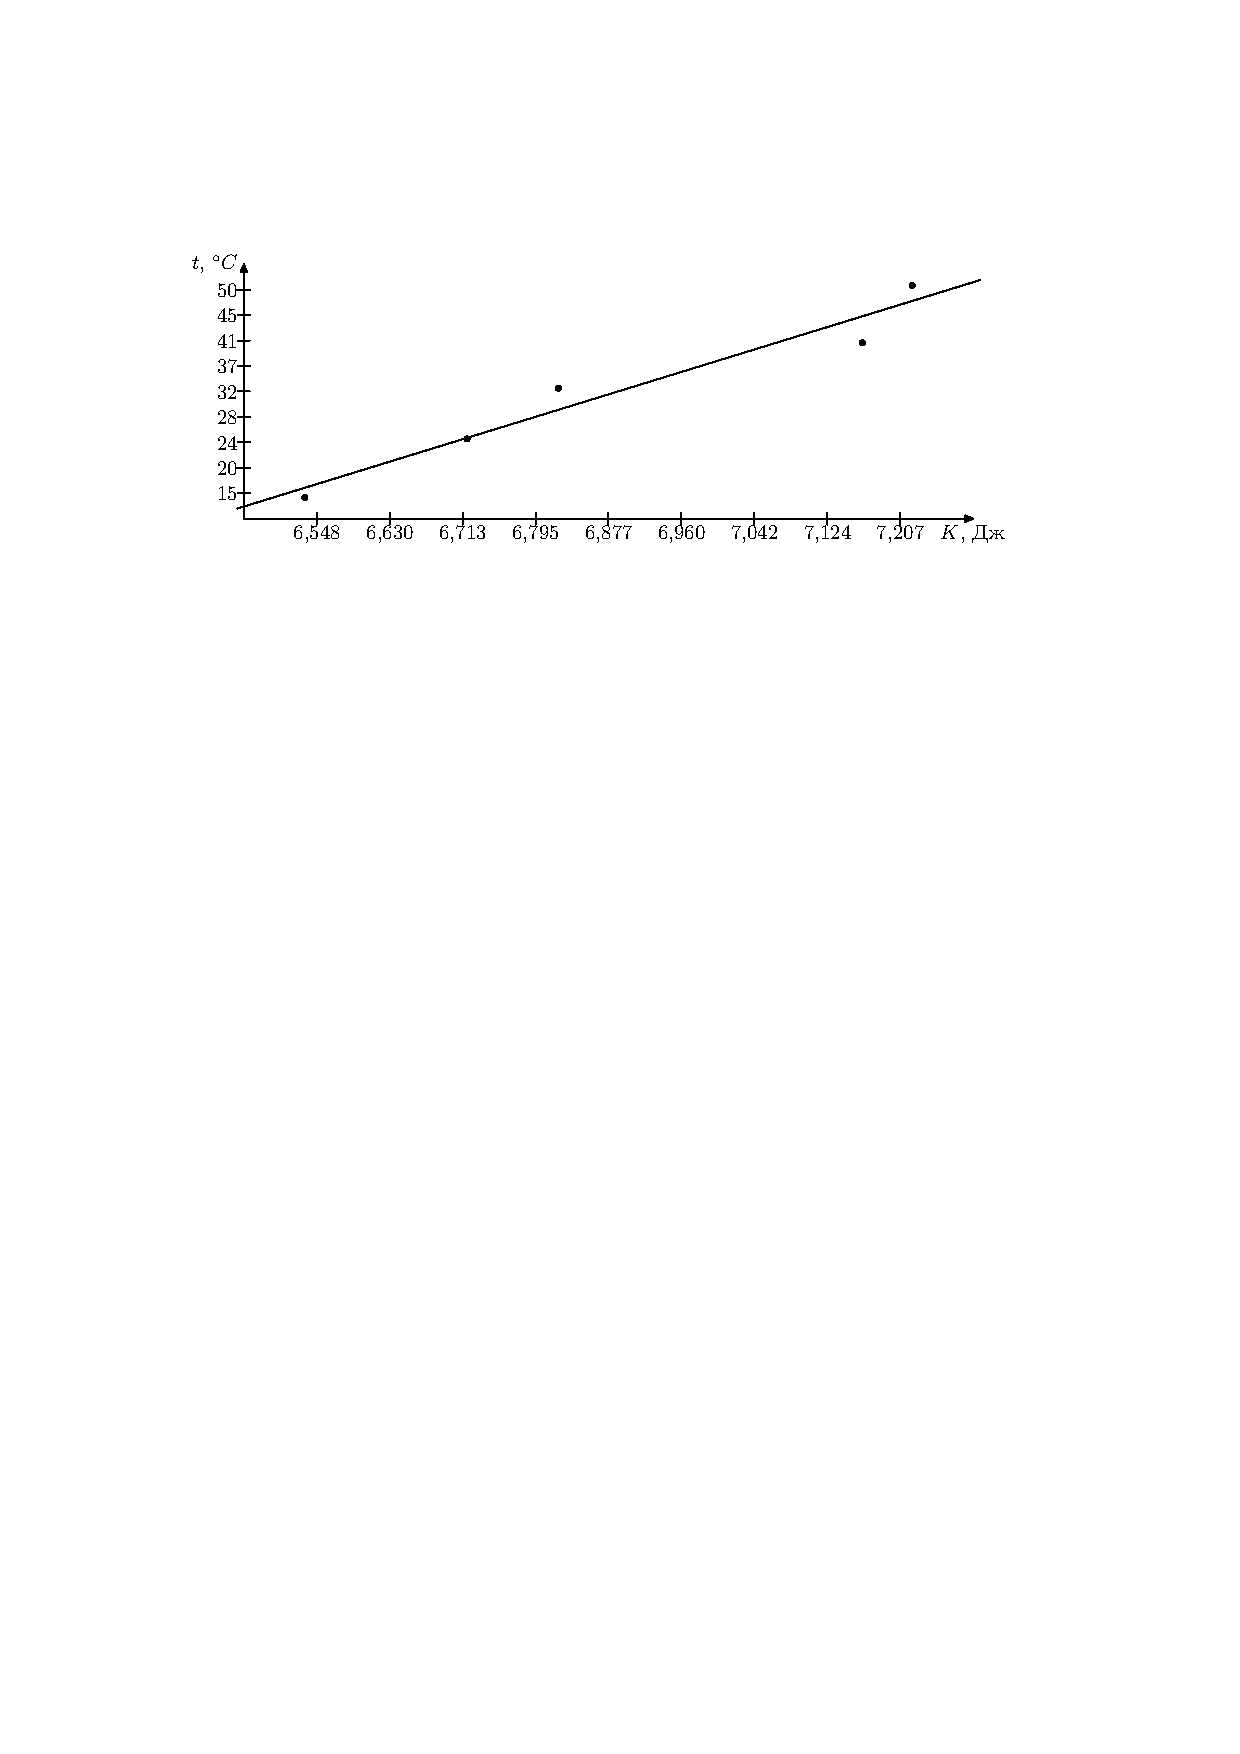
\includegraphics[scale=1]{pics/pdf/points2.pdf}
    \end{flushleft}

    Найти погрешности $\Delta A$, $\Delta C$ и 
    вычислить погрешность температуры абсолютного нуля:
    \begin{equation}
        \Delta t_0 = \sqrt{
            \left(\frac{\Delta A}{A}\right)^2 + 
            \left(\frac{\Delta C}{C}\right)^2
        } = 42{,}62^{\circ}C
    \end{equation}

    \item По данным таблиц 1.1--1.5 заполнить таблицу 2.2. 
    
    \begin{center}
        Таблица 2.2. Зависимость давления газа от температуры при разных 
        значениях объема

        \begin{tabular}{|@{$\,$}c@{$\,$}|@{$\,$}c@{$\,$}|@{$\,$}c@{$\,$}|@{$\,$}c@{$\,$}|@{$\,$}c@{$\,$}|@{$\,$}c@{$\,$}|@{$\,$}c@{$\,$}|@{$\,$}c@{$\,$}|@{$\,$}c@{$\,$}|@{$\,$}c@{$\,$}|@{$\,$}c@{$\,$}|}
\hline
$V_ц$, мл & 50 & 60 & 70 & 80 & 90 & 100 & 110 & 120 & 130 & 140\\
\hline
$t,\, {}^{\circ}C$ & \multicolumn{10}{c|}{$P$, кПа}\\
\hline
14,5 & 104,99 & 91,59 & 80,69 & 71,69 & 64,54 & 58,74 & 53,84 & 49,74 & 46,19 & 43,04\\
\hline
24,4 & 108,94 & 94,89 & 83,94 & 74,44 & 66,94 & 60,84 & 55,64 & 51,34 & 47,79 & 44,44\\
\hline
32,5 & 111,74 & 96,29 & 85,39 & 76,14 & 67,09 & 61,54 & 57,24 & 52,14 & 48,49 & 45,24\\
\hline
38,1 & 113,64 & 98,69 & 87,14 & 77,49 & 69,69 & 62,94 & 58,14 & 53,64 & 50,09 & 47,29\\
\hline
48,2 & 115,59 & 100,39 & 89,14 & 79,34 & 71,49 & 64,79 & 59,29 & 54,84 & 50,94 & 47,54\\
\hline
$\frac1{V_ц}$, мл${}^{-1}$ & 0,020 & 0,017 & 0,014 & 0,013 & 0,011 & 0,010 & 0,009 & 0,008 & 0,008 & 0,007\\
\hline
$\tilde{t}_0,\, {}^{\circ}C$ & -316,08 & -335,29 & -312,23 & -303,21 & -302,38 & -321,30 & -312,73 & -310,50 & -306,46 & -286,11\\
\hline
\end{tabular}
\par

    \end{center}
    
    Пользуясь таблицей 2.2 для значений объема цилиндра $50$, $90$, $140$ 
    мл на одной координатной сетке построить графики $P(t)$, убедиться, 
    что они <<идут>> прямолинейно.
    
    \begin{center}
        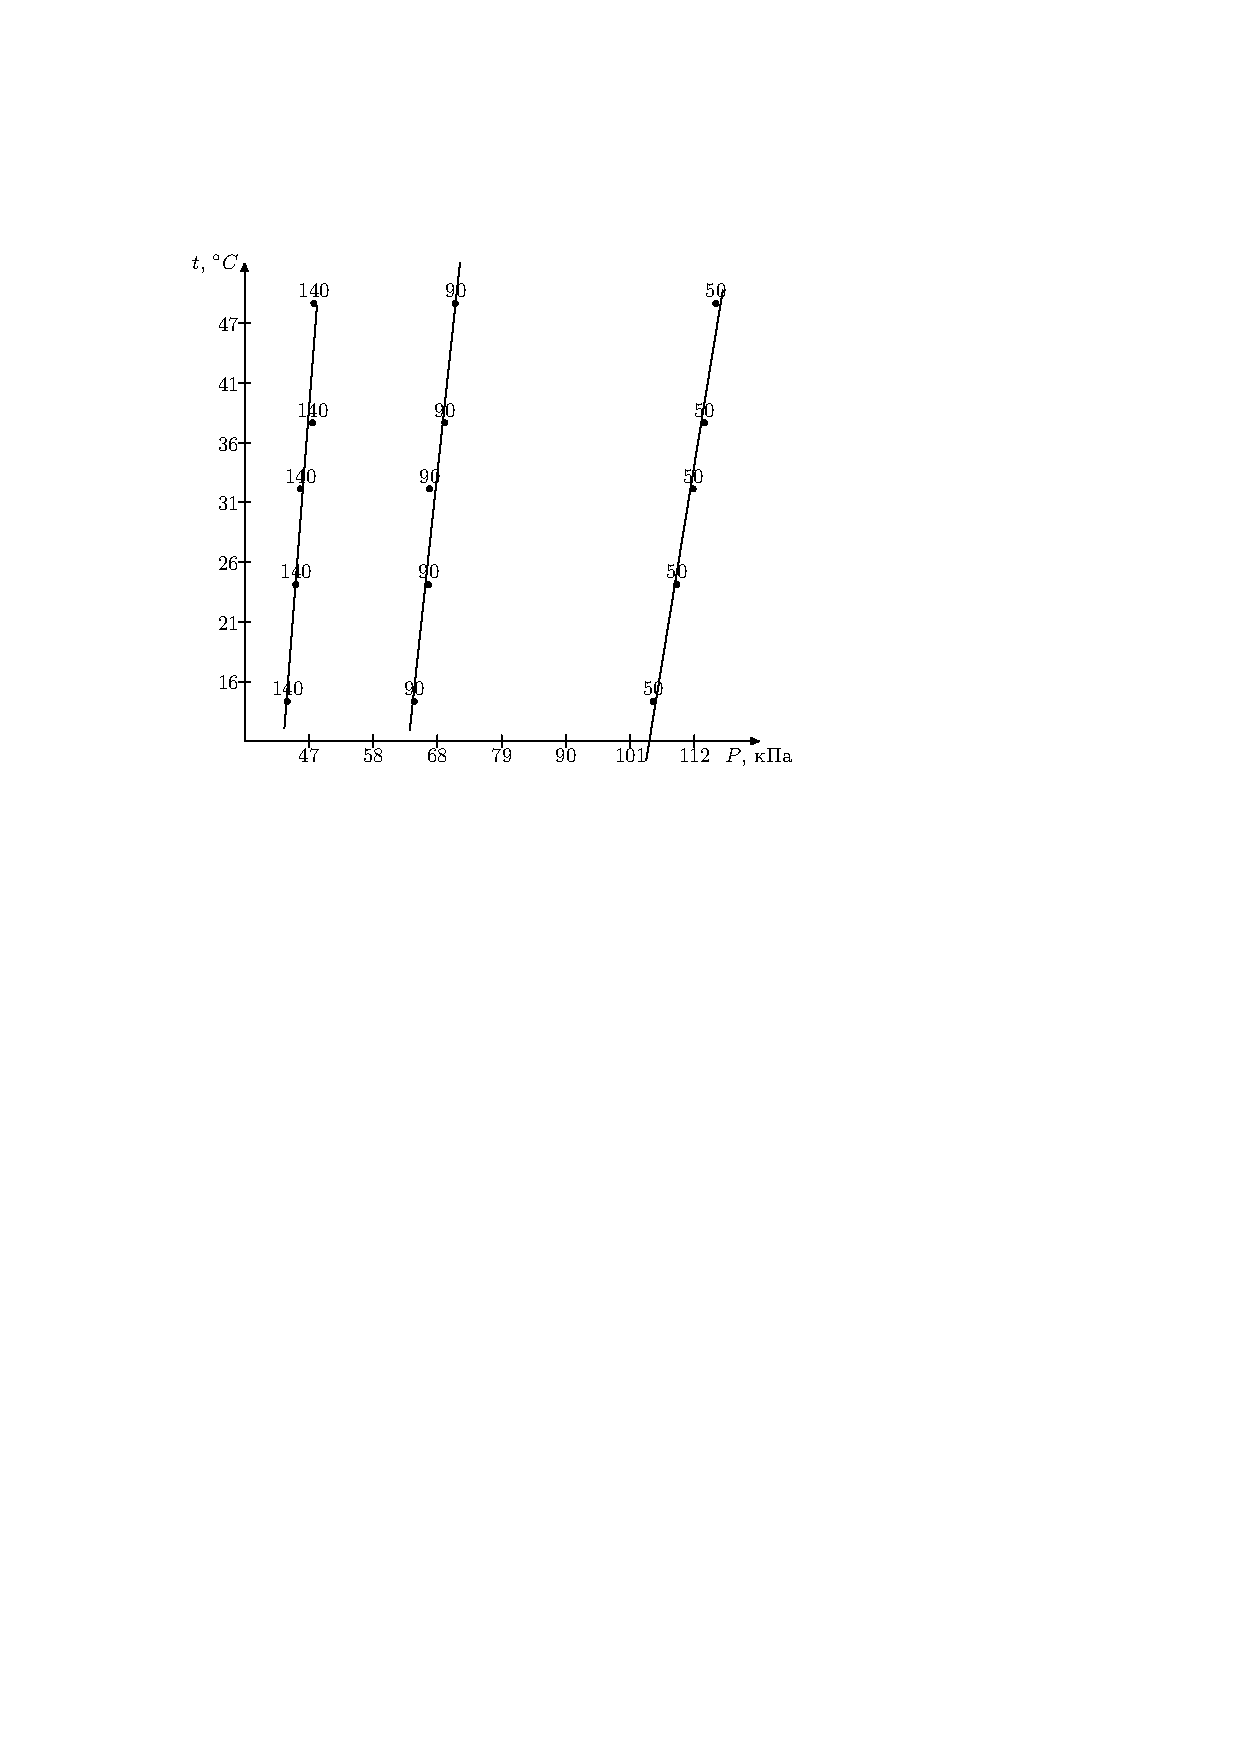
\includegraphics{pics/pdf/points3.pdf}
    \end{center}
    
    \item Для каждого из объемов в таблице 2.2 найти значение обратного 
    объема $\frac1{V_ц}$ и рассчитать величину $\tilde{t}_0$ по формуле
    \begin{equation}
        \tilde{t}_0 = - \frac{c}{a}
    \end{equation}
    где $a$ и $c$, соответственно, угловой коэффициент и свободное 
    слагаемое для зависимости $P(t)$.
    Занести значения в таблицу 2.2.
    
    \item Пользуясь таблицей 2.2, по формулам найти угловой коэффициент 
    $A'$ и свободное слагаемое $C'$ для зависимости $\tilde t_0(\frac1{V_ц})$. 
    Величина $C'$ фактически есть предел (\ref{lim}), т.е. совпадает со 
    значением $t_0$. На координатной сетке $\tilde t_*$ от $\frac1{V_ц}$ 
    отметить экспериментальные точки и начертить прямую, соответствующую 
    параметрам $A'$ и $C'$. Продолжить прямую до пересечения с осью ординат.

    \begin{center}
        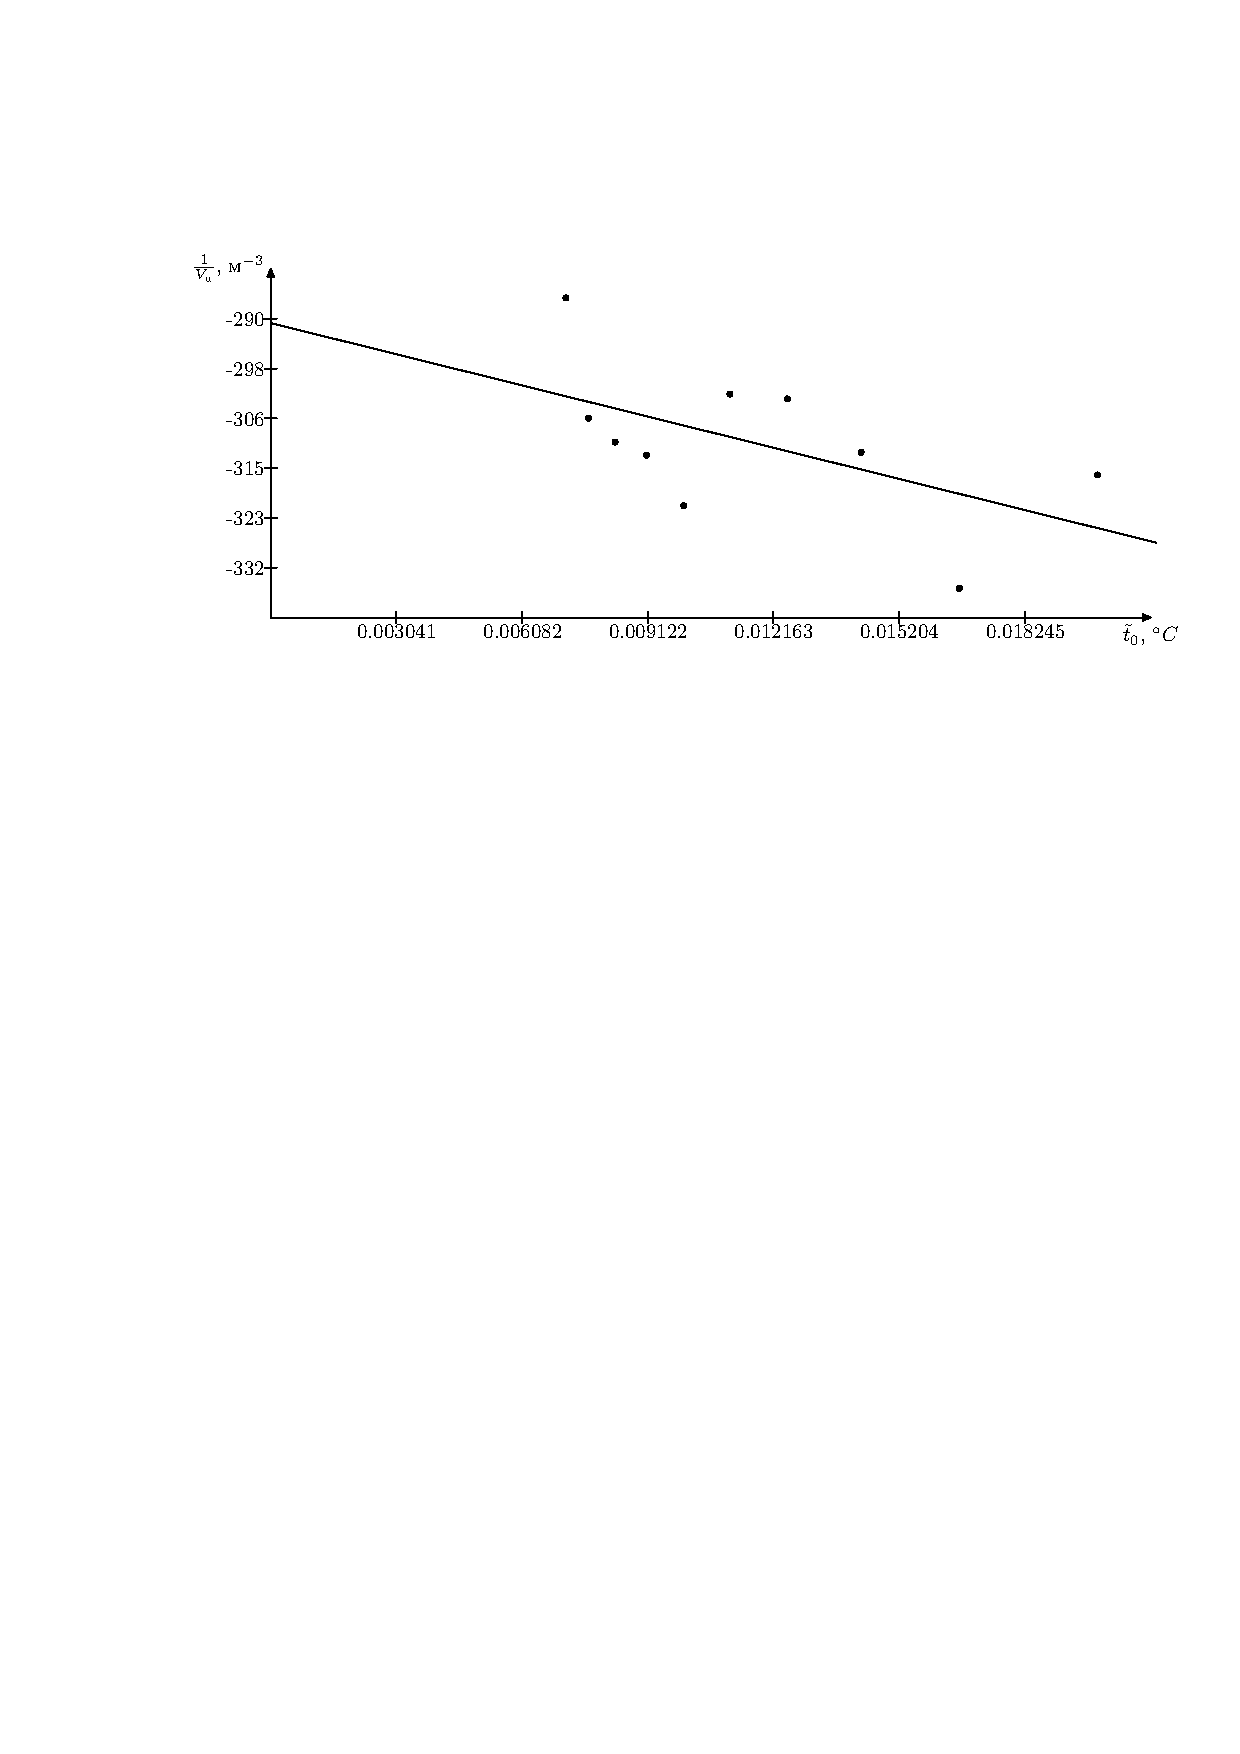
\includegraphics{pics/pdf/points4.pdf}
    \end{center}

    По этой зависимости, $t_0 = -290{,}36$
    
    \item Рассчитать погрешность $\Delta t_0$ как $\Delta C'$: 
    $\Delta t_0 = 11{,}06$
    
    \item Для нахождения аппроксимирующих прямых использовались 
    следующие формулы:
    \begin{equation}
        A = \frac1D \sum\limits_{i = 1}^N (X_i - \bar{X}) Y_i, \quad 
        C = \bar{Y} - A \bar{X}
    \end{equation}
    
    \begin{equation}
        \bar{X} = \frac1N \sum\limits_{i = 1}^N X_i, \ 
        \bar{Y} = \frac1N \sum\limits_{i = 1}^N Y_i, \ 
        D = \sum\limits_{i = 1}^N (X_i - \bar{X})
    \end{equation}
    
    \item Погрешности коэффициента и слагаемого вычисляются по формулам
    \begin{equation}
        \Delta A = \sqrt{\frac{E}{D}}, \quad 
        \Delta C = \sqrt{\left(\frac1N + \frac{\bar X^2}{D}\right) \cdot E}
    \end{equation}
    где
    \begin{equation}
        E = \frac{1}{N - 2} \sum\limits_{i = 1}^N (Y_i - AX_i - C)^2
    \end{equation}    

\end{enumerate}
